\documentclass{article}
\usepackage[utf8]{inputenc}
\usepackage{tikz}
\thispagestyle{empty}

\begin{document}
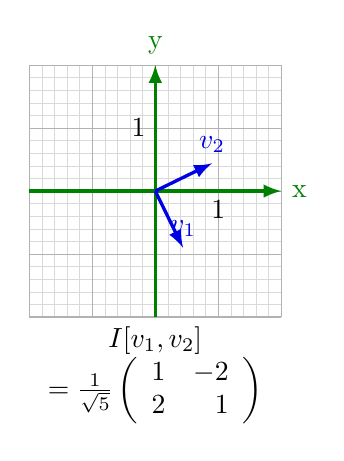
\begin{tikzpicture}[scale=0.8, samples=100, >=latex]
% Draw the coordinate frame
\def\range{2.}
\draw[step=0.2, very thin,color=gray!30!white] (-\range,-\range) grid (\range,\range);
\draw[step=1.0,color=gray!60!white] (-\range,-\range) grid (\range,\range);
\draw[->, >=latex, very thick, color=green!50!black] (-\range,0) -- (\range,0) node[right] {x};
\draw[->, >=latex, very thick, color=green!50!black] (0,-\range) -- (0,\range) node[above] {y};    
\draw (1, 0) node[left,below]{$1$};    
\draw (0, 1) node[below,left]{$1$};

% draw the vector:
\draw[->,color=blue!90!black, very thick] (0,0) -- (0.44, -0.9) node[above]{$v_1$};
\draw[->,color=blue!90!black, very thick] (0,0) -- (0.9, 0.44) node[above]{$v_2$};
\node [below,align=center] at (0,-\range) {$I [v_1,v_2]$\\ $= \frac{1}{\sqrt{5}} \left( \begin{array}{rr} 1 & -2 \\ 2& 1 \\ \end{array}\right)$};
\end{tikzpicture}
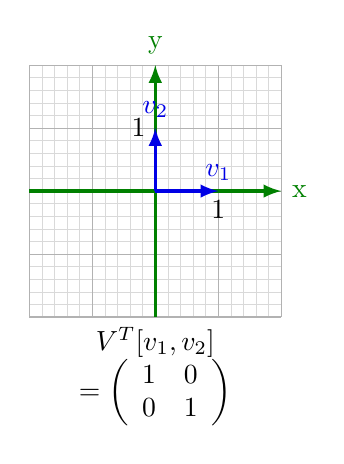
\begin{tikzpicture}[scale=0.8, samples=100, >=latex]

% Draw the coordinate frame
\def\range{2.}
\draw[step=0.2, very thin,color=gray!30!white] (-\range,-\range) grid (\range,\range);
\draw[step=1.0,color=gray!60!white] (-\range,-\range) grid (\range,\range);
\draw[->, >=latex, very thick, color=green!50!black] (-\range,0) -- (\range,0) node[right] {x};
\draw[->, >=latex, very thick, color=green!50!black] (0,-\range) -- (0,\range) node[above] {y};    
\draw (1, 0) node[left,below]{$1$};    
\draw (0, 1) node[below,left]{$1$};

% draw the vector:
\draw[->,color=blue!90!black, very thick] (0,0) -- (1,0) node[above]{$v_1$};
\draw[->,color=blue!90!black, very thick] (0,0) -- (0,1) node[above]{$v_2$};
\node [below,align=center] at (0,-\range) {$V^T [v_1,v_2]$\\ $=\left( \begin{array}{rr} 1 & 0 \\ 0& 1 \\ \end{array}\right)$};
\end{tikzpicture}
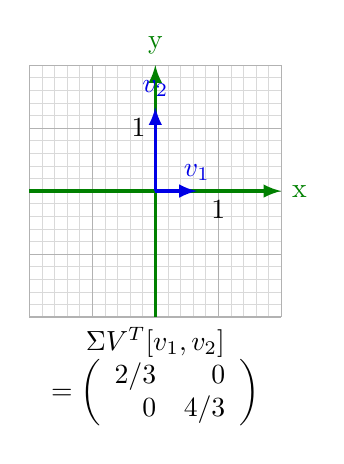
\begin{tikzpicture}[scale=0.8, samples=100, >=latex]

% Draw the coordinate frame
\def\range{2.}
\draw[step=0.2, very thin,color=gray!30!white] (-\range,-\range) grid (\range,\range);
\draw[step=1.0,color=gray!60!white] (-\range,-\range) grid (\range,\range);
\draw[->, >=latex, very thick, color=green!50!black] (-\range,0) -- (\range,0) node[right] {x};
\draw[->, >=latex, very thick, color=green!50!black] (0,-\range) -- (0,\range) node[above] {y};    
\draw (1, 0) node[left,below]{$1$};    
\draw (0, 1) node[below,left]{$1$};

% draw the vector:
\draw[->,color=blue!90!black, very thick] (0,0) -- (0.66, 0) node[above]{$v_1$};
\draw[->,color=blue!90!black, very thick] (0,0) -- (0, 1.33) node[above]{$v_2$};
\node [below,align=center] at (0,-\range) {$\Sigma V^T [v_1,v_2]$\\ $=\left( \begin{array}{rr} 2/3 & 0 \\ 0& 4/3 \\ \end{array}\right)$};
\end{tikzpicture}
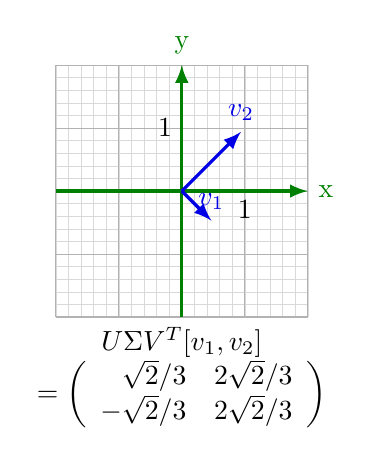
\begin{tikzpicture}[scale=0.8, samples=100, >=latex]

% Draw the coordinate frame
\def\range{2.}
\draw[step=0.2, very thin,color=gray!30!white] (-\range,-\range) grid (\range,\range);
\draw[step=1.0,color=gray!60!white] (-\range,-\range) grid (\range,\range);
\draw[->, >=latex, very thick, color=green!50!black] (-\range,0) -- (\range,0) node[right] {x};
\draw[->, >=latex, very thick, color=green!50!black] (0,-\range) -- (0,\range) node[above] {y};    
\draw (1, 0) node[left,below]{$1$};    
\draw (0, 1) node[below,left]{$1$};

% draw the vector:
\draw[->,color=blue!90!black, very thick] (0,0) -- (0.47, -0.47) node[above]{$v_1$};
\draw[->,color=blue!90!black, very thick] (0,0) -- (0.94, 0.94) node[above]{$v_2$};
\node [below,align=center] at (0,-\range) {$U \Sigma V^T [v_1,v_2]$\\ $=\left( \begin{array}{rr} \sqrt{2}/3 & 2\sqrt{2}/3 \\ -\sqrt{2}/3& 2\sqrt{2}/3 \\ \end{array}\right)$};
\end{tikzpicture}

\end{document}